\chapter{Infrastructure}\label{sec:infra}

Many points of contention had to be resolved when developing the game's infrastructure. Most notably, what the agent teams wanted it to look like from a technical point of view. It was decided to keep the infrastructure as generic and open-ended as possible, empowering the agents to have as much control over the game as possible. At the same time, a single reality had to be maintained by a trusted source to prevent agents from creating and spreading fundamental untruths. These constraints led to a compromise of decisions that are outlined in this chapter and the rationale behind them.

\section{Design Decisions}
One of the larger design decisions we took was to use the Go language for this task. This was taken after much deliberation over what language provides the best features compared to their perceived cost. Strong arguments were made for languages such as Elixir which has an in-built messaging protocol and Python which is very familiar to most people. In the end, Go was chosen because of its performance, type safety, excellent concurrency and tooling with clear error messages and the ability to check for data races and deadlocks before running the program.

\section{Agent Design}
As mentioned, agents are entities that are spawned at the start of discussion rounds or when action is required. By doing this, the game can utilise parallelism to scale to thousands of agents whilst performing acceptably. At the same time, communication channels are maintained between each of the other agents to allow messages to be sent whenever an agent deems it necessary.
Agents all have a BaseAgent and a Strategy. The BaseAgent is shared among all agents and contains fields such as a view of the state of the game, and the agent's own latest state (as determined by the game). Meanwhile, the Strategy is where all the core decision-making of a strategy is made. This includes methods to implement decision-making for the Fight, Election, Loot, HPPool and Trade stages of the game.


\section{Data Availability}
To ensure a consistent source of truth, the game must make sure that all the information the agents receive about the game is correct. Normally this is done by passing values to agents by copy instead of by reference. However, in the case of arrays and maps, in Go, these are always passed by reference. This is a problem because agents do not have the permission or power to change any of the realities that they are experiencing.

Instead, an immutable library is used to create immutable views of these lists and maps. In doing so we can pass these arrays and maps, which are key to the functionality of the game, around to all of the agents without fear of them being changed which could cause a data race at best.

\section{Communication}
Agents communicate through implemented message interfaces. These give agents the option to send various types of messages depending on the state of the game - however, whether agents choose to understand or respond to a given message is up to them. To provide protection from potential deadlocks or data races, direct channel access is abstracted away from agent implementation.

A big concern raised was that using the concurrent model, agents would not know how long to wait before moving on to another message. This is a serious problem as basing it on time would mean that the game is slowed down significantly to wait for these timeouts to pass, whilst basing it on a messaging limit would favour performant agents that can send out more messages (even with the assumption of no malice).

The compromise chosen was to have two different types of messages - Request and Inform messages. Request messages are those where the sender expects an answer immediately. Of course, this time may be variable in code, but this means that an agent can wait for the return value from another agent's message handler. Inform messages on the other hand do not return a value so the sender knows not to wait for anything.

This solution provides a suitable compromise to increase simulation performance and remove the need for excessive timeouts at the cost of reduced flexibility in communication and more methods to implement in the Strategy interface.

\section{Proposals}
Proposals happen during the Election stage or at the start of every fight round. Agents are requested to put forward proposals to the elected leader which is done using Ostrom's ADICO grammar \cite{OstromADICO}.

If a proposal is voted on or chosen by a leader, then the allocated action is sent to each agent. Agents then have the choice to follow the action or defect. By choosing the latter they are subject to be put on a defector list to be seen by all and subject to social sanctions from their peers.

\section{Trading}
Trading is another significant technical part of the game. They are fundamentally asynchronous but are implemented as a series of rounds between agents but validated by the game to ensure everything is sound. The process involves one agent starting a negotiation and then the receiver can accept, decline or negotiate.

Figures \ref{fig:trade_game} and \ref{fig:trade_agent} show what this stage looks like from the point of view of the game and from the two agents involved in the negotiation.

\begin{figure}[htb]
    \centering
    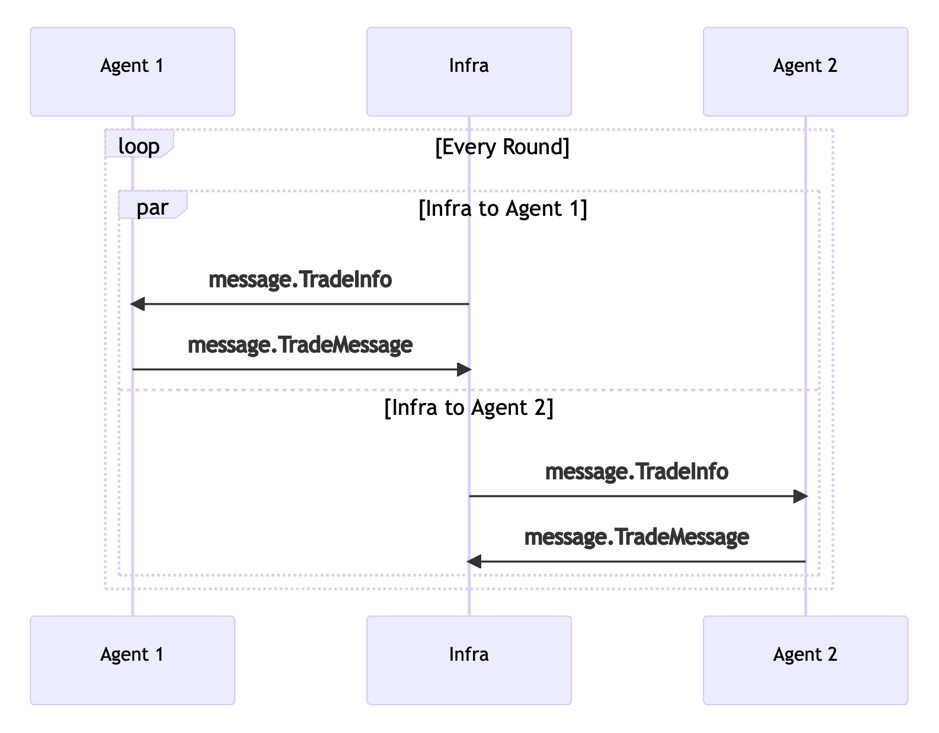
\includegraphics{003_infrastructure/images/trade1.png}
    \caption{The game's perspective}
    \label{fig:trade_game}
\end{figure}

\begin{figure}[htb]
    \centering
    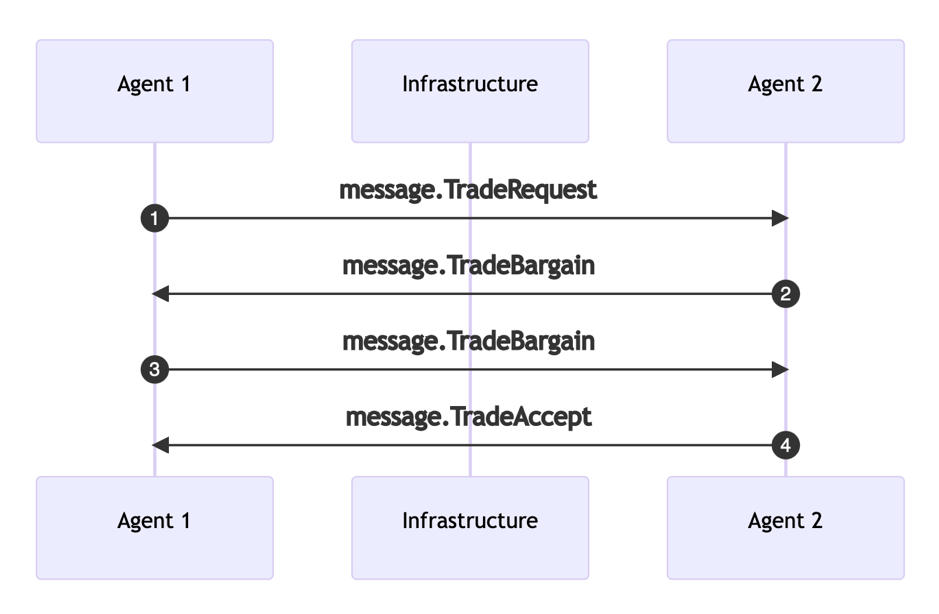
\includegraphics{003_infrastructure/images/trade2.png}
    \caption{The agent's perspective}
    \label{fig:trade_agent}
\end{figure}

\section{Web}
To complement the game and make it easier for teams to evaluate their agent's performance across many games, a front-end was also implemented. This gave teams the opportunity to run many experiments.

Running on an AWS EC2 instance, the front end features 2 main views: the `Configuration' and the `Result' view. The configuration view enables the user to configure any of the starting parameters such as the starting values and the number of each type of agent. Meanwhile, the result view allows the team to see the details about their run including the git commit and graphs about both the entire game state and the internal agent state of any of the agents within the game (as well as the distribution of values across a class of agents). Additionally, logs were also provided to be downloaded if the agent teams wanted to conduct further analysis of the data.

These logs were stored in a MongoDB cloud instance to be able to be easily shared among teams and compare results both on a micro- and macro-scale.
